\chapter{Process View}

The process view, as the name indicates, corresponds to the previously documented
process viewpoint. As such, it is mostly targeted at the system developer and, in part,
to the project manager categories of stakeholders. To some extent, it can also be of
use to the system administrator stakeholder, for a better understanding of the
interactions in the system.

\section{Overview of processes}

The first series of models in the process view (figure \ref{fig:cop_0}, figure \ref{fig:cop_1},
figure \ref{fig:cop_2}, figure \ref{fig:cop_3}) illustrates the highest level configuration
of the processes existing in the system. Each of the figures describe this configuration
at a particular phase in the evolution of the system.

\begin{figure}[ht]
\begin{center}
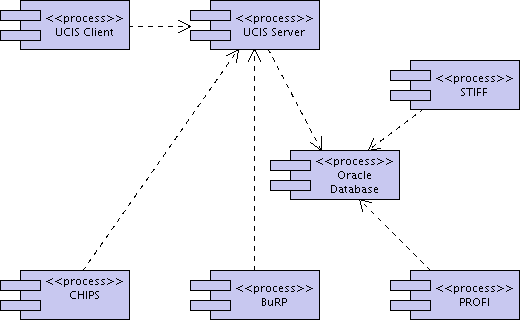
\includegraphics[width=3in]{img/cop_0.png}
\end{center}
\caption{Configuration of processes, phase 0}
\label{fig:cop_0}
\end{figure}

As can be seen, figure \ref{fig:cop_0} shows the processes in the system in phase 0 of
development (the current state of the system). Note that in this phase UCIS is divided
in a client and a server process, with each client process running on a separate machine
(currently, machines used by the Call-Center employees) and the server process running
on a single machine (currently located in the central headquarters in Amsterdam).
Another relevant thing to notice is that the STIFF process provides no means of interaction
for the other processes. Use of the STIFF process is done solely by means of the Oracle
database, both in order to make proposal computation requests and to collect results.

\begin{figure}[ht]
\begin{center}
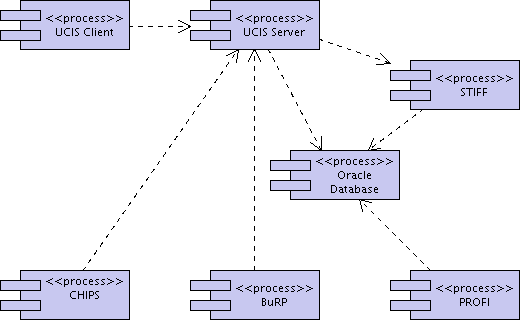
\includegraphics[width=3in]{img/cop_1.png}
\end{center}
\caption{Configuration of processes, phase 1}
\label{fig:cop_1}
\end{figure}

This problem is addressed in two steps: first, in phase 1, a simple wrapper around STIFF is
to be provided, which will allow direct interaction of the other systems (particularly UCIS)
with it. This modification is envisioned at this earliest phase since it:
\begin{itemize}
\item{involves a very small amount of work;}
\item{can contribute significantly to an increase in the productivity of the company, since a
proposal could thus be computed right away, instead of having to wait 24h for it to become
available.}
\end{itemize}

The second step involves a full rewrite of the STIFF system in Java, again making sure that
it can accept requests from other systems. Since this implies a lot more work than the first
step, it is only planned to be finished by the end of phase 3 (see development view). The
difference to be noticed between the phase 0 configuration of processes and the other phases
is the additional line connecting UCIS to STIFF, which implies STIFF's availability for direct
requests (i.e., no longer through the Oracle database).

\begin{figure}[ht]
\begin{center}
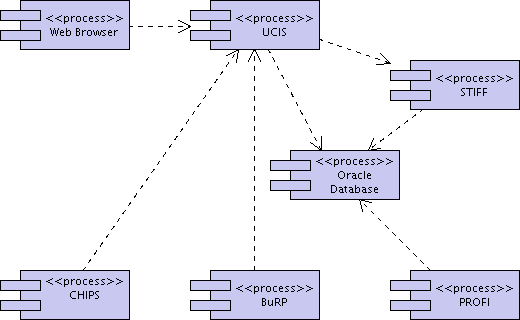
\includegraphics[width=3in]{img/cop_2.png}
\end{center}
\caption{Configuration of processes, phase 2}
\label{fig:cop_2}
\end{figure}

Another difference to be noticed between phase 1 configuration and phase 2 configuration is
that UCIS is transformed from a traditional, proprietary protocol, client/server system to a
web-based client/server system, with the old client/server processes from figure \ref{fig:cop_1}
being replaced by the new browser/web server processes from figure \ref{fig:cop_2}. This
transformation is justified by two requirements:
\begin{itemize}
\item{the requirement to provide web-based access for customers;}
\item{the (implicit) requirement to refactor the UCIS system so that the entire business logic
runs on the server, leaving only the presentation layer for the client (browser) to handle.}
\end{itemize}

Going from phase 2 to phase 3 implies, in terms of processes, the introduction of the GOC process
which is to be used for generating all output. This means that all the requests for various types
of output which are made through the PROFI and the UCIS system will no longer be handled by
the respective process, but will instead be forwarded to the GOC process. This modification comes
to meet the requirement that all output has to be done through the GOC component by the
end of 2005. Also in phase 3 the STIFF process is supposed to be rewritten completely in Java,
using a multithreaded design, but this is not visible at this higher level. This distinction is, however,
made clear in the next section.

\begin{figure}[ht]
\begin{center}
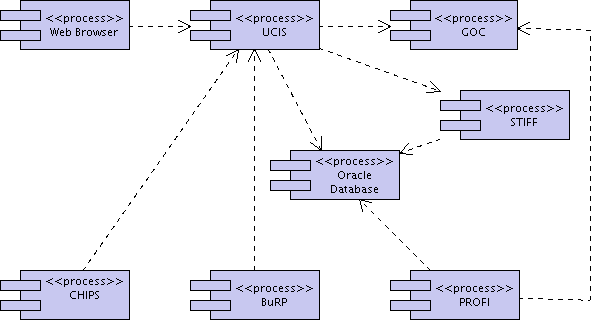
\includegraphics[width=3.5in]{img/cop_3.png}
\end{center}
\caption{Configuration of processes, phase 3}
\label{fig:cop_3}
\end{figure}

\section{Process interaction}

This section goes into slightly more detail about how the processes described in the previous
section actually interact. As our topmost quality requirement is interoperability, we show here
how the processes (are supposed to) interact at the end of each of the three phases in the evolutionary
development of the system. Throughout, we try to point out by means of the diagrams how
interoperability is ensured at each phase of development.

\begin{figure}[ht]
\begin{center}
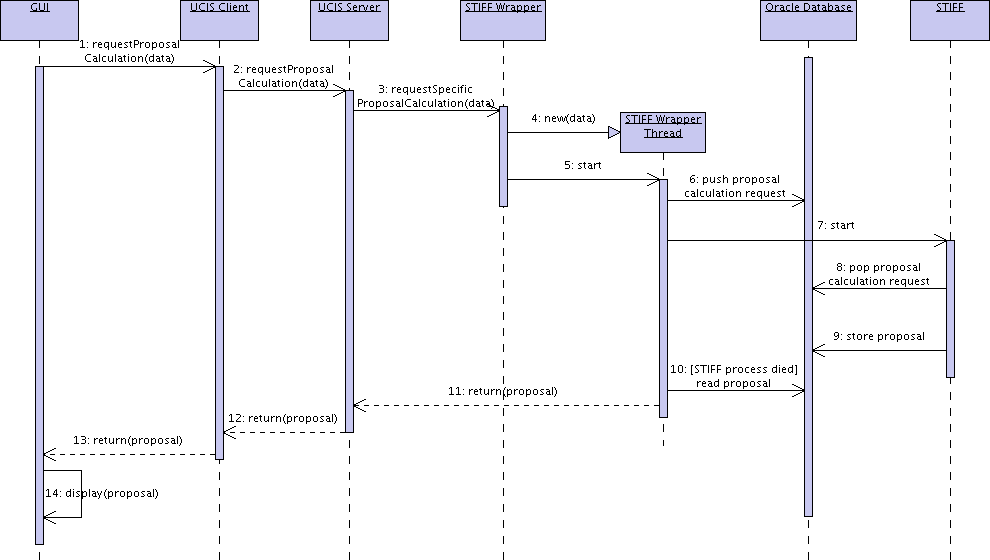
\includegraphics[width=\linewidth]{img/pi_1.png}
\end{center}
\caption{Process interaction, phase 1}
\label{fig:pi_1}
\end{figure}

Process interaction at the end of phase 1 is illustrated in figure \ref{fig:pi_1}. Here, the Call-Center
employee requests a proposal calculation by means of the GUI. Existing proprietary protocol
communication takes place over TCP/IP between the UCIS Client and the UCIS Server. When the
request arrives, the UCIS server calls the newly introduced (in this phase) STIFF Wrapper, making
a request for a specific proposal calculation (after previous interpretation of the generic request
made by the client). The wrapper will start a thread for handling the request. This thread will
then conduct the process described below to get the proposal and then return it to the UCIS server.
The UCIS server will send the result back to the UCIS client, again by using a proprietary protocol
over TCP/IP. Here is, then, the process by which the wrapper thread conducts the calculation:

\begin{enumerate}
\item The wrapper thread places the proposal data in the Oracle Database, marking it as uncomputed
(e.g. by setting a boolean value).
\item The wrapper thread starts the STIFF system.
\item STIFF will run as before, i.e. it will read all entries in the proposal table and will check if any
of them have to be computed (e.g. by looking at the boolean value), make all computations, and
place the result(s) back into the database. All wrapper threads will have to coordinate so that only
one instance of STIFF is started. Any of the common synchronization mechanisms (locks, semaphores,
etc.) can be used for this purpose. The reason why we don't want more than one instance of STIFF
to be started is because otherwise we might have two or more instances of STIFF computing the same
proposal which, especially since the used algorithms are so complex, would be counter-efficient.
\item The wrapper waits for STIFF to end execution and then reads the results from the database
and returns them to the UCIS Server.
\end{enumerate}

In terms of process interaction, the only changes brought by phase 2 are that the UCIS system no
longer communicates using a proprietary protocol, but instead by using HTTP. This is a consequence
of the UCIS system becoming a web-based system as the main change of phase 2. This can be seen
in figure \ref{fig:pi_2}. Although depicted in the diagram, you are referred to \cite{fow03} for a
complete description of the \textit{Front Controller} pattern (which is what is used here in order to handle
HTTP requests), where you can find all the necessary information also in what the process itself is
concerned. The reason for using the \textit{Front Controller} pattern in this system is because we want to
be able to handle any common task (e.g. authentication) in a single place instead of having to duplicate
it for each separate page which the UCIS provides.

\begin{figure}[ht]
\begin{center}
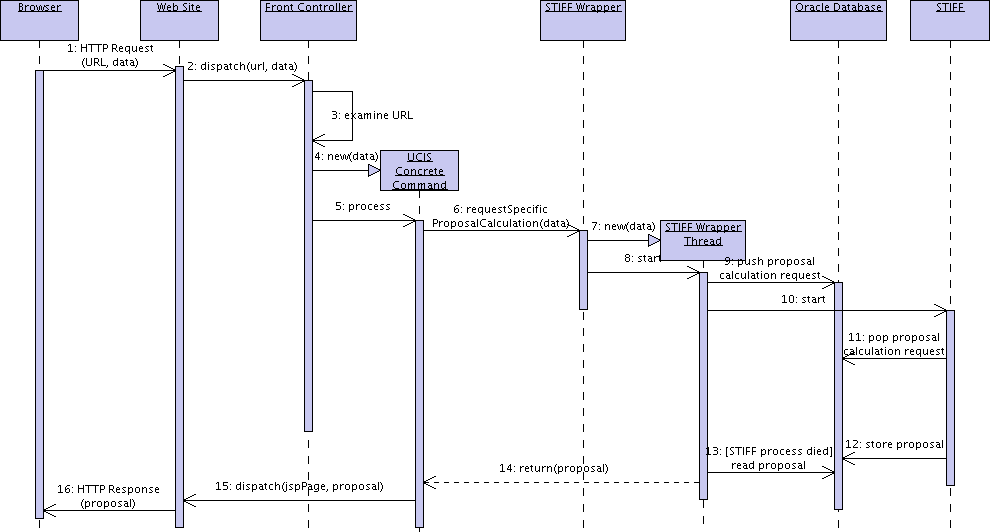
\includegraphics[width=\linewidth]{img/pi_2.png}
\end{center}
\caption{Process interaction, phase 2}
\label{fig:pi_2}
\end{figure}

As a remark, in what the UCIS system is concerned, it will naturally run as a multithreaded system,
but all multithreading/synchronization issues are fully handled by the J2EE application server, so
details about such issues are not provided in this document as they are not seen as being part of the
application itself. On the other hand, for scalability reasons, UCIS is to be modified (if necessary) in such a way that
multiplication of the whole system on any number of machines is possible. This implies that any
session information has to be stored in the database so that clustering can be done in a transparent
manner. More explicitly, a (possible) load balancer might (and probably will, due to randomness)
dispatch requests pertaining to the same logical session to different instances of the UCIS server. By
using the \textit{Database Session State} pattern this can be easily handled so that it does not
become an issue. For further information on the aforementioned pattern, you are referred to \cite{fow03}.

Finally, the process interaction by the end of phase 3 is shown in figure \ref{fig:pi_3}, where you can
see that communication with the STIFF process can now be done in a much easier way, as we no longer
need the wrapper. As also mentioned in the logical view, by the end of phase 3, STIFF is expected to
have been completely rewritten in Java, using RMI to make itself available for direct requests from
the UCIS at any time. The reason for choosing RMI is that by using it, all inter-process communication
is simplified to mere remote method invocations, which allows for faster (and also cheaper) development.
An additional argument supporting the decision to use RMI is that the amount of communication (measured
here as the number of remote calls) that is needed is quite small (one remote call per customer request),
so then the performance of the overall system will not suffer due to an otherwise significant delay entailed
by remote calls. This loose dynamic coupling (i.e. small number of remote calls) between UCIS and STIFF,
combined with our resolve of achieving a high degree of scalability, also explains why we are placing STIFF
on different machines than UCIS. As a remark, notice that the process (involving the STIFF Wrapper)
described as necessary in phases 1 and 2 can now be discarded altogether, as it is no longer needed.

\begin{figure}[ht]
\begin{center}
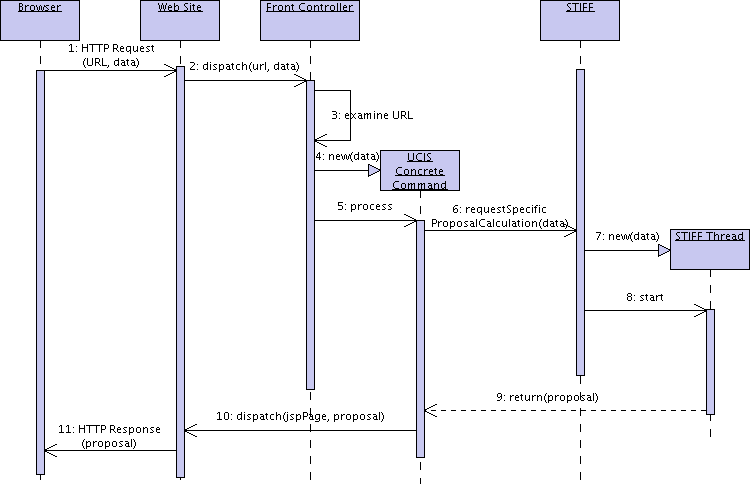
\includegraphics[width=\linewidth]{img/pi_3.png}
\end{center}
\caption{Process interaction, phase 3}
\label{fig:pi_3}
\end{figure}

\section{The STIFF System}
\label{sec:pv_stiff}

Last but not least, as one of our main goals is scalability and as scalability comes into play especially
when discussing the STIFF system (since this is the part of the whole application with the largest
processing needs), it is essential that the rewriting of STIFF in Java (planned for the 3\textsuperscript{rd}
phase of development) meets the following requirements:

\begin{itemize}
\item any number of STIFF processes can be run in parallel on any number of machines (to ensure
scalability), without any need for communication between them (to ensure transparency);
\item STIFF processing is done in a multi-threaded manner so there is a chance, when STIFF runs on
multi-processor machines, that separate threads can be scheduled by the operating system to run on
different processors, thus allowing for scalability of the number of processors.
\end{itemize}

\begin{figure}[ht]
\begin{center}
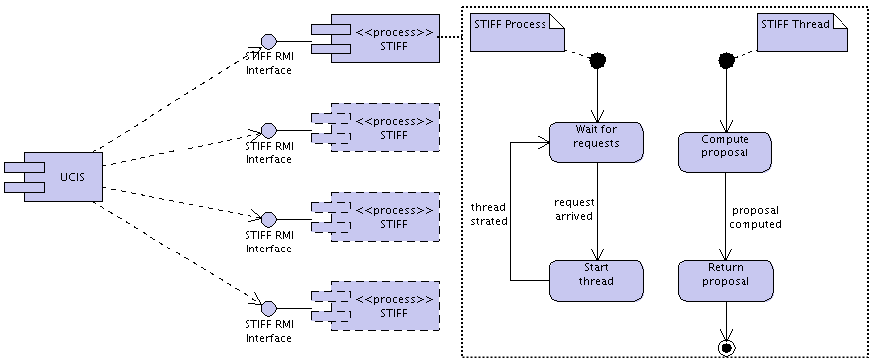
\includegraphics[width=\linewidth]{img/stiff.png}
\end{center}
\caption{Overview of the final STIFF system}
\label{fig:stiff}
\end{figure}

The first requirement implies that no synchronization is necessary between STIFF processes. This
is feasible as each proposal calculation is essentially independent of the others and as now UCIS
makes proposal requests directly to STIFF (i.e., not by setting values in the Oracle database). The
latter means that the danger that more STIFF processes/threads might compute the same request
for a proposal calculation no longer exists (as we expect UCIS to properly coordinate what request
goes to what STIFF system).

The second requirement has already been briefly mentioned in figure \ref{fig:pi_3}, where we show
the main STIFF process spawning a new thread to deal with each request. Achieving this is also
necessary in order to meet the response time quality attribute which we have set as a goal. By having
multiple threads we expect that the average response time will be increased due to possible parallel
processing (on multi-processor machines).

Figure \ref{fig:stiff} summarizes this discussion, while the physical view completes it with scalability
aspects which are relevant from the physical viewpoint.